\documentclass[utf8,a4paper]{article}
\usepackage[UTF8,noindent]{ctex}	%	太好了。从Beamer学到的,居然在这里用上了。
\setCJKmainfont[ItalicFont={KaiTi},BoldFont={SimHei}]{SimSun}
\setCJKsansfont{SimHei}
\setCJKmonofont{FangSong}
\usepackage{graphicx}
\usepackage[top=30mm,left=3.0cm,bottom=2.5cm,right=2.5cm]{geometry}

\usepackage{listings}%	源代码
%\usepackage{booktabs}		专为三线表

\usepackage{makecell}		%控制横线粗细的好选择

\usepackage{hyperref}	%	提供autoref	好东西

% Title Page
\title{\textbf{\sffamily Experiment Report of Computer Architecture}\\  \begin{large}\sffamily Build a New Linux Kernel Image(3.12) for ARM ISA in gem5 FS Mode \end{large}
}

%\subtitle{}
\author{Lei Zungjyun\\李颂元\\21321293 \and Anqing Zhao\\赵安清\\21321047}
\CTEXoptions[today=old]
\begin{document}
\maketitle

\begin{abstract}
This article is an experiment report of the computer architecture course. 
\end{abstract}

\section{Introduction}
	\subsection{Overview}
	In FS (Full System) mode, gem5 can boot an entire operating system such as Linux. However, the kernel images offered by gem5 official site are relatively old (kernel version 2.x). We built a new kernel (3.12) that can be booted by gem5. gem5 supports several ISA such as Alpha, ARM, x86, etc. We built a kernel for ARM and run it on gem5 for ARM, as illustrated in \autoref{fig:arc}.


	\begin{figure}[htbp]
		\centering
		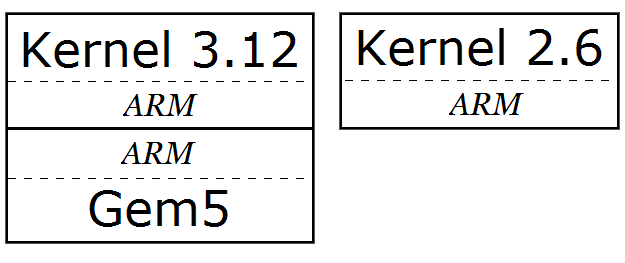
\includegraphics[width=0.5\textwidth]{images/arch2.png}
		\caption{Architecture}\label{fig:arc}	%label要贴在caption旁边,不然会出错
	\end{figure}
	\subsection{Steps}\label{text:steps}
		Here are the steps we follow to accomplish the experiment.
		\begin{enumerate}
			\item
			Install requisite packages.
			\item
			Download gem5 and compile it for ARM version.
			\item
			Download Linux kernel and cross-compile it for ARM version.
			\item
			Configur M5\_DIR.
			\item
			Run and test.
		\end{enumerate}
		First of all, we should install some packages on our experiment computer. These packages are necessary for buiding kernel and gem5. After downloading gem5 from \url{gem5.org} and Linux kernel (3.12) from \url{kernel.org}, we should compile them for ARM version. Here is how we built the gem5 for ARM version.
\begin{lstlisting}[language=bash, frame=shadowbox]
scons build/ARM/gem5.opt 
\end{lstlisting}

Notice that the Linux kernel will be run on an ARM machine, which is different from our experiment platform, so we should build the kernel with cross-compiling. Here is how we cross-compiled the Linux kernel.
\begin{lstlisting}[language=bash, frame=shadowbox]
make ARCH=arm O=PATH menuconfig
make ARCH=arm CROSS_COMPILE=arm-linux-gnueabi- O=PATH vmlinux-3.12
\end{lstlisting}
Then, we can configure the M5\_DIR, which contains kernel image (vmlinux-3.12) and disk image (linux-arm-ael.img). Finally, we can run the new kernel on gem5 and check it with m5term, which is a virtual terminal of gem5.
		
	\subsection{Environment}
	We use a computer in our lab to compile Linux and run gem5 for testing new-version Linux. The machine's performance is a bit low, so it brings some trouble to us. \autoref{tab:env} shows our environment.

\begin{table}[htbp]
	\caption{Hardware and operating system}\label{tab:env}
	\centering
	\begin{tabular}{c|cc}
		\Xhline{2pt}
		Device	&	\multicolumn{2}{c}{Optiplex GX620}\\
		\Xhline{1pt}
				&	CPU				&	Pentium D 3.00GHz X 2	\\
				&	Memory			&	2GB\\
		\Xhline{1.5pt}
		OS		&	\multicolumn{2}{c}{Ubuntu 13.04} \\
		\Xhline{1pt}
				&	ISA				&	AMD64\\
				&	Swap			&	2GB\\
		\Xhline{2pt}
	\end{tabular}
\end{table}

\section{Obstacles and Solutions}
We face to problems as soon as we start to do the experiment.
	\subsection{Compiling Errors}
		\subsubsection{gem5}
The first time we build gem5, we use
\begin{lstlisting}[language=bash, frame=shadowbox]
scons build/ARM/gem5.opt -j2.
\end{lstlisting}
to obtain the thread-level parallelization, but the system got stuck. We opened the system monitor and we found that the 2GB-DRAM was used out and the swapping area was also used out. This meaned the compiling of gem5 is memory-intensive and therefore we compiled it serially. This turn, the DRAM was used out again but the swapping area was not. Finally, the compiling was finished, although the compiling time was nearly one hour and a half.
		\subsubsection{Kernel}
			As we said in the \autoref{text:steps}, we shold notice the cross-compiling.  The documentation of the Linux kernel warned us that if we do not install the prerequisite packages first, we will fall in a trap that we can not turn back, so we should check the necessary packages seriously before we build the kernel.

	\subsection{Runtime Errors}
		\subsubsection{gem5}
				SE (Syscall Emulation) mode runs smoothly.
		\subsubsection{Kernel}
	We must explicitly assign a memory size before we run the gem5 for ARM in FS mode. The size can not be larger than 256MB. We conject that this rule is designed for the emulation of embedded system serveral years ago when the RAM of the embedded system was relatively small. If the developer does not assign a memory size explicitly, the gem5 will use arbitrary size of the host computer which can be much larger than the target embedded system. Therefore, gem5 make this rule for ARM version.

\subsection{Methodology}
We have no much experience in compiling a new-version Linux for ARM. During studying and trying, we countered various problems and wierd situations. To find the answesr, effective methods should be used.
	\begin{enumerate}
		\item
		Classification: Tutorials.
		\item
		Index: Google.
		\item
		Compromise: Documentation and videos.
	\end{enumerate}
As the documentation of gem5 are arranged in a wiki way, it is a compromise of classification and index.
\section{Result}
We can type
\begin{lstlisting}[language=bash, frame=shadowbox]
build/ARM/gem5.opt -d /tmp/output configs/example/fs.py \
	--kernel=vmlinux-3.12 --mem-size=256MB
\end{lstlisting}
in  the shell to run the gem5 and type
\begin{lstlisting}[language=bash, frame=shadowbox]
util/term/m5term 3456
\end{lstlisting}
to monitor the gem5.


After booting, we can type root to enter the default account. Then we typed
\begin{lstlisting}[language=bash, frame=shadowbox]
uanme -a
\end{lstlisting}
to show the system information. The result screenshot is showed in \autoref{fig:result}.
\begin{figure}[htbp]
\centering
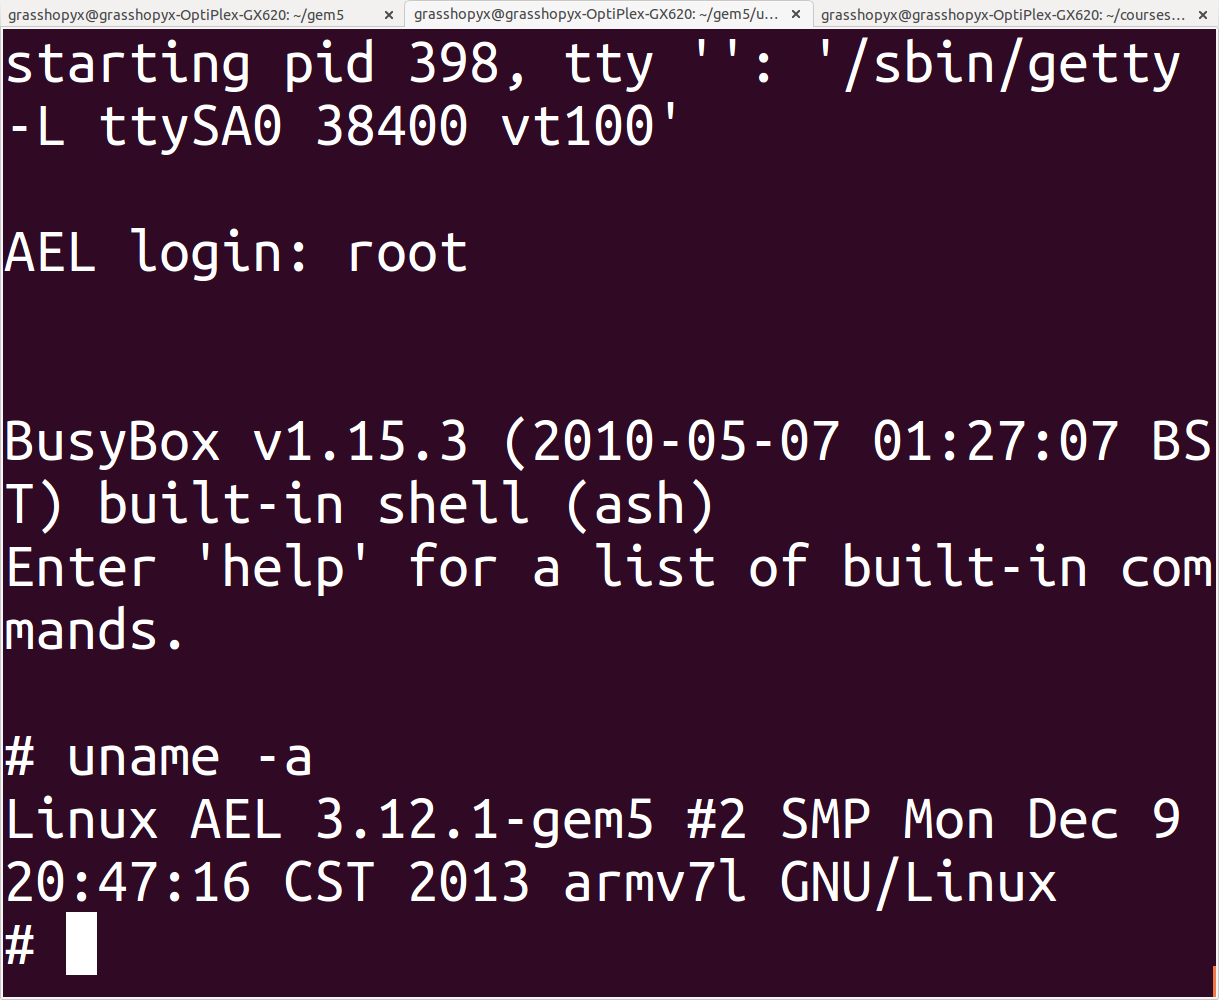
\includegraphics[width=0.7\textwidth]{images/result.png}
\caption{Result Screenshot}\label{fig:result}
\end{figure}
	
\section{Cooperation}
This task can hardly be done in a divide-and-conquering way. We discuss and solve the problems together and get the ideal result eventually.

\section{Acknowlegements}
Prof. 陈文智 offered us this opportunity to do the experiment. Doctor 卢忠勇, who is the teahing assistant, guided us to do that. Doctor 谢斌 and doctor 叶敏娇 helped us to overcome some obstacles. Mark Chen, zxz and other friends on the Internet also enlightened us to finish this experiment. Thank you very much!

\end{document}